\documentclass[conference]{IEEEtran}
\usepackage{fontspec}
\setmainfont{lmroman10-regular.otf}
\setsansfont{lmsans10-regular.otf}
\setmonofont{lmmono10-regular.otf}
\usepackage{graphicx}
\usepackage{booktabs}
\usepackage{amsmath}
\usepackage{amssymb}
\usepackage{url}
\usepackage{array}
\renewcommand{\abstractname}{Streszczenie}
\renewcommand{\refname}{Literatura}
\renewcommand{\IEEEkeywordsname}{Słowa kluczowe}

\title{Benchmark gotowych systemów ASR na polskim dyktowaniu radiologicznym: terminologia, liczby i błędy istotne klinicznie}

\author{\IEEEauthorblockN{Konrad Strojny}\IEEEauthorblockA{E-mail: \texttt{konrad.j.strojny@gmail.com}}}

\begin{document}
\maketitle

\begin{abstract}
Gotowe systemy automatycznego rozpoznawania mowy (ASR) są coraz częściej rozważane do dyktowania opisów radiologicznych, jednak ich zachowanie na polskiej mowie klinicznej jest słabo scharakteryzowane. Porównano 19 gotowych systemów (12 konfiguracji otwartych i 7 komercyjnych usług chmurowych) na 939 nagraniach naturalnego głosu (2,69\,h, 14 mówców) z zakresu ultrasonografii tarczycy oraz radiologii głowy i szyi. Poza wskaźnikami WER (word error rate) i CER (character error rate) mierzona jest przede wszystkim poprawność \emph{terminologii} radiologicznej (TER, term error rate) wobec słów ogólnych (GWER) oraz błędy w liczbach, zaprzeczeniach i stronie ciała, podsumowane wskaźnikiem błędów istotnych klinicznie (CCER). W klasycznych modelach ASR terminy są rozpoznawane 3--6$\times$ gorzej niż słowa ogólne; transkrybery oparte na dużych modelach językowych (LLM) zmniejszają tę lukę. Najlepszy model otwarty (Whisper large-v3) myli 15,8\% wystąpień terminów, ale tylko 3,1\% słów ogólnych; najlepsza usługa chmurowa (OpenAI gpt-4o-transcribe) osiąga WER 5,96\%, a Google Gemini 3.5 Flash ma najniższy TER (6,6\%). Konwencje zapisu liczb mogą istotnie zawyżać surowy WER, dlatego obok niego podawany jest WER znormalizowany pod względem liczb. Wyższy odsetek błędów dla terminów utrzymuje się także przy tej samej częstości słowa, więc nie wynika wyłącznie z rzadkości słów.
\end{abstract}

\begin{IEEEkeywords}
automatyczne rozpoznawanie mowy, język polski, radiologia, dyktowanie medyczne, terminologia, benchmark
\end{IEEEkeywords}

\section{Wprowadzenie}
Radiolodzy coraz częściej dyktują opisy do systemów rozpoznawania mowy. Ogólne modele, takie jak Whisper, dobrze radzą sobie z mową potoczną, jednak w dyktowaniu radiologicznym mylą się częściej na terminologii, liczbach i jednostkach, skrótach oraz nazwach własnych. Błędy w opisie badania obrazowego nie są sobie równe: jedne są kosmetyczne (interpunkcja, końcówki fleksyjne), inne zmieniają znaczenie kliniczne i mogą pozostać niezauważone przez lekarza---podmieniona strona ciała („prawy'' $\to$ „lewy''), zły wymiar („45\,mm'' $\to$ „4\,mm''), zgubione zaprzeczenie („bez zmian'' $\to$ „zmian'') albo słowa wstawione, których nikt nie wypowiedział (tzw. halucynacje).

\noindent\textbf{Pytania badawcze.}
\begin{enumerate}
\item Jak duży jest błąd rozpoznawania (WER, CER) polskich fraz z opisów radiologicznych dla gotowych rozwiązań ASR: modeli otwartych uruchamianych lokalnie i komercyjnych usług chmurowych?
\item Jak poprawnie zapisywane jest słownictwo radiologiczne (anatomia, opis obrazu, jednostki chorobowe i zabiegi, skróty i nazwy obce) w porównaniu ze słowami ogólnymi w tych samych nagraniach? Jakiego rodzaju są to błędy: fleksja, podział na słowa, błędna pisownia słyszanego terminu, podmiana na inne słowo, pominięcie?
\end{enumerate}

\noindent\textbf{Wkład pracy.}
\begin{itemize}
\item Benchmark 12 konfiguracji otwartych (10 modeli otwartych, w tym warianty z modelem językowym i kontrola negatywna) oraz 7 komercyjnych usług chmurowych na 939 nagraniach radiologicznych naturalnego głosu.
\item Analiza błędów na poziomie terminów, oddzielająca terminy (309 form w czterech klasach) od słów ogólnych przez TER i GWER, z klasyfikacją błędów na fleksję, podział, bliski zapis, podmianę i pominięcie.
\item Kategorie istotne klinicznie (liczby, zaprzeczenia, strona ciała), połączony wskaźnik CCER oraz przybliżenie halucynacji (wstawki co najmniej trzech słów).
\item WER znormalizowany pod względem liczb (WER-N), oddzielający błędy rozpoznania od konwencji zapisu liczb.
\end{itemize}

\section{Powiązane prace}
Oceniane modele otwarte wprowadzono we wcześniejszych pracach: Whisper \cite{r2}, wav2vec 2.0 \cite{r3} oraz wielojęzyczna rodzina MMS \cite{r4}. Nowsze transkrybery dziedzinowe i komercyjne opisano w ich kartach modeli i dokumentacji produktowej (Sekcja~\ref{sec:evaluated}). Benchmarki ASR dla dyktowania klinicznego koncentrowały się głównie na języku angielskim i na zagregowanym WER; niniejsza praca dotyczy polskiego dyktowania radiologicznego i analizuje błędy na poziomie pojedynczych terminów oraz tokenów istotnych klinicznie (liczby, zaprzeczenia, strona ciała).

\section{Dane}
\subsection{Nagrania badawcze}
Wykorzystano 939 nagrań polskiej radiologii naturalnego głosu (2,69\,h, 14 mówców): krótkie czytane frazy z opisów USG tarczycy oraz głowy i szyi, a nie spontaniczne dyktowanie całych opisów. Nagrania pochodzą z publicznego korpusu badawczego (ADMEDVOICE; Kaggle \texttt{karmarci/polish-medical-multi-source-corpus}, DOI 10.34740/kaggle/ds/6698205, licencja CC~BY~4.0) \cite{r1}; wykorzystano wyłącznie wariant naturalnego głosu ludzkiego.

\subsection{Podzbiór radiologiczny}
Z ośmiu kategorii tematycznych korpusu zachowano dwie kategorie radiologiczne: \texttt{02-001} (USG tarczycy) i \texttt{02-003} (głowa i szyja). Zbiór testowy obejmuje 939 nagrań naturalnych (2,69\,h, 14 mówców, 246 tekstów). Czasy wyliczono z nagłówków plików WAV. Frazy mają od 2 do 46 słów, średnio 15,8. Ten sam mówca czyta ten sam tekst wielokrotnie (129 przypadków, 258 nagrań); żadne dwa pliki audio nie są identyczne (MD5), a metadane sprawdzono pod kątem błędów kategorii (61 nagrań jednego mówcy przeniesiono z \texttt{02-001} do \texttt{02-003}).

\section{Metody}
\subsection{Etapy badania}
Każdy system otrzymuje wyłącznie nagranie i informację, że językiem jest polski. Nie stosuje się promptów ze słownictwem, list słów kluczowych, słowników niestandardowych, kontekstu medycznego ani korekty po rozpoznaniu (etap „bez pomocy''). Jedynym wyjątkiem jest Google Gemini (ogólny LLM), który wymaga polecenia tekstowego i otrzymuje neutralną instrukcję „przepisz dosłownie'', bez słownictwa i bez wzmianki o medycynie.

\subsection{Oceniane systemy}\label{sec:evaluated}
\noindent\textbf{Modele otwarte (offline).} Whisper medium, large-v3-turbo i large-v3 \cite{r2}; NVIDIA Canary-1B-v2 \cite{r5}, NVIDIA Parakeet-TDT-0.6B-v3 \cite{r6} i Qwen3-ASR-1.7B \cite{r8}; NVIDIA FastConformer PL \cite{r7}; wav2vec2 XLSR-53 Polish \cite{r3,r9} oraz Meta MMS-1b-all \cite{r4}, każdy bez modelu językowego i z ogólnym polskim KenLM \cite{r20}; a także Google MedASR \cite{r10}, model tylko angielski, jako kontrola negatywna.

\noindent\textbf{Usługi chmurowe (online).} OpenAI whisper-1 i gpt-4o-transcribe \cite{r11}, ElevenLabs Scribe v2 \cite{r12}, Deepgram Nova-3 \cite{r13}, AssemblyAI Universal-2 \cite{r14}, Speechmatics (polski) \cite{r15} oraz Google Gemini 3.5 Flash \cite{r16}.

\subsection{Procedura}
Zbiór testowy jest przepróbkowany do 16\,kHz mono. Dekodowanie jest identyczne w obrębie rodziny modeli, bez promptów i słowników. Whisper używa dekodowania zachłannego z \texttt{language=pl}, \texttt{task=transcribe}, fp16 na GPU Maca (MPS) \cite{r2,r17}. Modele CTC (wav2vec2, MMS) używają dekodowania zachłannego; warianty „+KenLM'' stosują beam search (pyctcdecode) z ogólnym polskim 5-gramowym modelem językowym z repozytorium \texttt{jonatasgrosman/wav2vec2-large-xlsr-53-polish} \cite{r9,r19,r20}. Modele NVIDIA NeMo używają domyślnego dekodera (Canary z \texttt{source\_lang=target\_lang=pl}). Każde nagranie chmurowe wysyłane jest osobnym żądaniem (WAV 16\,kHz mono, \texttt{language=pl}) z do 8 żądań równolegle; usługi asynchroniczne są odpytywane, a ich pliki i zadania usuwane po odczytaniu transkrypcji.

\subsection{Normalizacja tekstu i metryki}
Normalizacja tekstu (taka sama dla referencji i hipotezy) zmienia litery na małe, usuwa interpunkcję, rozdziela wymiary („14x12x45'' $\to$ „14 x 12 x 45''), odkleja jednostki („50mm'' $\to$ „50 mm''), zachowuje przecinek dziesiętny i usuwa znaczniki techniczne. Liczby \emph{nie} są zamieniane na słowa.

Metryki liczone są biblioteką jiwer \cite{r18}: WER i CER z 95\% przedziałem ufności z bootstrapu po wypowiedziach (1\,000 losowań); WER-N (WER po zamianie liczb na słowa za pomocą num2words \cite{r23}, „x''$\to$„na'' i jednostek słownych na skróty); oraz trzy kategorie istotne klinicznie---liczby (tokeny z cyfrą), zaprzeczenia („nie'', „bez'', „brak'') i strona ciała (formy prawy/lewy)---jako odsetek błędnie rozpoznanych tokenów referencji (podmiana lub pominięcie). \textbf{CCER} (clinically critical error rate) to jeden wskaźnik ważony liczbą tokenów (mikro-uśredniony) po trzech kategoriach:
\begin{equation}
\mathrm{CCER} = 100\cdot\frac{\text{num\_err}+\text{neg\_err}+\text{side\_err}}{\text{num\_n}+\text{neg\_n}+\text{side\_n}},
\end{equation}
liczony po łącznej puli 2\,988 tokenów krytycznych (1\,990 liczb, 399 zaprzeczeń, 599 tokenów strony ciała). Każdy token liczony jest raz; liczą się tylko podmiany i pominięcia, spójnie z pojedynczymi kategoriami. Wstawki $\ge 3$ kolejnych słów przybliżają halucynacje. RTF (real-time factor) to czas przetwarzania podzielony przez długość audio (MacBook Pro M1 Pro, 16\,GB); RTF usług chmurowych obejmuje sieć i kolejkę i nie jest bezpośrednio porównywalny.

\subsection{Rozpoznawanie terminologii}
Słownik referencji zbioru testowego liczy 736 typów słów bez cyfr; oznaczono go w całości względem ręcznego leksykonu z jedną z czterech klas (Tabela~\ref{tab:lex}). Na wyrównaniu słów jiwer każde wystąpienie słowa referencji otrzymuje jeden status, sprawdzany w kolejności: poprawne; podział na słowa; pominięcie; fleksja (ten sam lemat, inna forma; lematy hipotezy z simplemma \cite{r22}); bliski zapis (odległość Levenshteina na znakach $\le \max(1, \mathrm{round}(0.3\cdot\text{długość}))$, o ile nie zmienia się przedrostek niosący znaczenie, co liczy się jako podmiana); podmiana. TER to odsetek wystąpień terminów o statusie innym niż \emph{poprawne}; TER-L liczy tylko bliski zapis, podmianę i pominięcie; GWER to ten sam wskaźnik dla słów ogólnych; iloraz TER/GWER mówi, ile razy trudniejsze są terminy. Błędy liczone są także w przedziałach częstości słów w ogólnej polszczyźnie (skala Zipfa; wordfreq \cite{r21,r24}).

\section{Wyniki}
\subsection{Modele otwarte}
Tabela~\ref{tab:wer-open} podaje WER i kategorie kliniczne. Whisper large-v3 jest najlepszym modelem otwartym (WER 8,03\%), także wobec nowszych modeli z lat 2025--2026. CCER potwierdza ranking, ale ujawnia ryzykowne klinicznie przypadki: Whisper large-v3 ma najniższy CCER wśród modeli otwartych (2,71\%), blisko swoich trzech wskaźników kategorii; Qwen3-ASR osiąga znacznie wyższy CCER (9,27\%) niż jego niski odsetek błędów liczb (7,7\%) z powodu częstych błędów zaprzeczeń (10,3\%) i strony ciała (13,7\%). Nowe modele NVIDIA tracą głównie na zapisie liczb (20--26\% w wymiarach); po normalizacji zapisu (WER-N 14--15\%) zbliżają się do Whisper medium. Ogólny polski model językowy poprawia modele CTC (wav2vec2 58,3$\to$52,8\%, MMS 35,2$\to$32,1\%). FastConformer PL myli stronę ciała w 37\% przypadków. MedASR, tylko angielski, daje WER $\sim$100\%, zastępując polską mowę angielskimi terminami medycznymi.

\begin{table*}[t]
\centering
\caption{Modele otwarte (offline). Wartości w procentach; WER z 95\% CI. Liczby, Zaprzeczenia, Strona ciała: odsetek błędnie rozpoznanych tokenów w kategorii (n = 1\,990/399/599); CCER łączy trzy kategorie po 2\,988 tokenach.}
\label{tab:wer-open}
\resizebox{\textwidth}{!}{%
\begin{tabular}{lcccccccccc}
\toprule
Model & WER [95\% CI] & WER-N & CER & Liczby & Zaprzecz. & Strona & CCER & Wstawki$\ge$3 & RTF \\
\midrule
Whisper large-v3 & 8.03 [7.43--8.73] & 7.61 & 2.17 & 2.8 & 2.8 & 2.5 & 2.71 & 2 & 0.139 \\
Whisper large-v3-turbo & 9.75 [9.1--10.44] & 9.21 & 2.57 & 2.8 & 1.5 & 2.8 & 2.61 & 3 & 0.082 \\
Whisper medium & 13.77 [12.94--14.64] & 13.12 & 3.94 & 4.1 & 2.5 & 3.8 & 3.85 & 6 & 0.071 \\
NVIDIA Parakeet-TDT-0.6B-v3 & 18.21 [17.2--19.2] & 15.03 & 6.29 & 20.8 & 1.8 & 5.3 & 15.13 & 3 & 0.097 \\
NVIDIA Canary-1B-v2 & 20.05 [18.95--21.34] & 14.04 & 8.66 & 25.6 & 1.5 & 5.0 & 18.27 & 8 & 0.295 \\
Qwen3-ASR-1.7B & 21.8 [20.9--22.76] & 18.35 & 7.37 & 7.7 & 10.3 & 13.7 & 9.27 & 3 & 0.151 \\
Meta MMS-1b-all (pol) + KenLM & 32.07 [30.88--33.35] & 25.72 & 12.47 & 81.8 & 1.8 & 6.8 & 56.09 & 13 & 0.101 \\
Meta MMS-1b-all (pol adapter, bez LM) & 35.22 [33.87--36.48] & 27.46 & 13.17 & 57.3 & 6.3 & 11.0 & 41.23 & 36 & 0.088 \\
NVIDIA FastConformer PL (hybrydowy, P\&C) & 50.7 [49.26--52.17] & 31.4 & 30.29 & 100.0 & 7.5 & 37.1 & 75.03 & 41 & 0.03 \\
wav2vec2 XLSR-53 Polish + KenLM & 52.8 [51.22--54.3] & 32.94 & 29.54 & 100.0 & 14.0 & 20.7 & 72.62 & 132 & 0.066 \\
wav2vec2 XLSR-53 Polish (bez LM) & 58.31 [56.67--59.69] & 41.08 & 30.68 & 100.0 & 23.8 & 25.5 & 74.90 & 121 & 0.07 \\
Google MedASR & 99.65 [99.21--100.08] & 99.01 & 80.48 & 98.2 & 100.0 & 100.0 & 98.83 & 41 & 0.011 \\
\bottomrule
\end{tabular}}
\end{table*}

\subsection{Usługi chmurowe}
Tabela~\ref{tab:wer-cloud} podaje usługi chmurowe. OpenAI gpt-4o-transcribe jest najlepszym systemem ogólnie (WER 5,96\%, CER 2,03\%, WER-N 4,47\%, najniższy odsetek błędów liczb 1,9\%); 54\% jego wypowiedzi jest bezbłędnych. Gemini 3.5 Flash zapisuje terminy najlepiej (TER 6,6\%) i ma najlepszy WER-N (4,18\%) oraz najmniej błędów zaprzeczeń (1,0\%), kosztem wyższego surowego WER z powodu „wygładzania''. Według CCER gpt-4o-transcribe jest najbezpieczniejszy klinicznie (2,07\%), a Gemini 3.5 Flash blisko (2,74\%), podczas gdy ElevenLabs Scribe v2 ma najwyższy CCER wśród usług chmurowych (65,56\%): zapisuje liczby słownie („2\,mm'' $\to$ „dwóch milimetrów''), co zawyża surowy WER do 28,27\% (WER-N 5,22\%) i czyni liczby źródłem błędów krytycznych, mimo niskiego TER.

\begin{table*}[t]
\centering
\caption{Usługi chmurowe (online). Kolumny jak w Tabeli~\ref{tab:wer-open}; RTF obejmuje sieć i kolejkę i nie jest porównywalny z modelami lokalnymi.}
\label{tab:wer-cloud}
\resizebox{\textwidth}{!}{%
\begin{tabular}{lcccccccccc}
\toprule
Model & WER [95\% CI] & WER-N & CER & Liczby & Zaprzecz. & Strona & CCER & Wstawki$\ge$3 & RTF \\
\midrule
OpenAI gpt-4o-transcribe & 5.96 [5.4--6.52] & 4.47 & 2.03 & 1.9 & 2.0 & 2.7 & 2.07 & 1 & 0.021 \\
OpenAI whisper-1 & 9.93 [9.26--10.62] & 9.45 & 2.58 & 3.5 & 3.3 & 3.5 & 3.48 & 1 & 0.032 \\
AssemblyAI Universal-2 & 10.25 [9.54--10.96] & 9.71 & 2.77 & 3.5 & 2.8 & 3.8 & 3.48 & 1 & 0.265 \\
Google Gemini 3.5 Flash & 10.4 [9.75--11.09] & 4.18 & 4.03 & 3.0 & 1.0 & 3.0 & 2.74 & 8 & 0.076 \\
Deepgram Nova-3 & 15.06 [14.3--15.84] & 8.48 & 7.88 & 8.0 & 3.5 & 2.5 & 6.33 & 6 & 0.018 \\
Speechmatics (pl) & 19.41 [18.68--20.18] & 16.37 & 6.18 & 16.1 & 0.3 & 7.0 & 12.18 & 1 & 0.03 \\
ElevenLabs Scribe v2 & 28.27 [26.22--30.33] & 5.22 & 23.53 & 97.7 & 1.3 & 1.7 & 65.56 & 65 & 0.037 \\
\bottomrule
\end{tabular}}
\end{table*}

\subsection{Terminologia radiologiczna}
Tabele~\ref{tab:ter-open} i~\ref{tab:ter-cloud} podają TER i jego rozkład. Terminy są 3,4--5,7$\times$ trudniejsze niż słowa ogólne dla klasycznych modeli z GWER $\le$ 10,2\%. Dominuje bliski zapis: u Whisper large-v3 8,7 z 15,8 punktów procentowych TER to bliskie zapisy („TIRADS''$\to$„TIRAC''/„TIRATS''/„TIRAS'', 104 ze 176 wystąpień; „color''$\to$„kolor''; „miąższ''$\to$„miosz''), czyli model słyszy termin, ale nie zna jego pisowni. Skróty i nazwy obce to najtrudniejsza klasa (Tabela~\ref{tab:class}). Wyjątkiem jest ElevenLabs Scribe v2, dla którego terminy są łatwiejsze niż słowa ogólne (TER/GWER 0,7, jedyny system poniżej 1,0). Efekt dziedziny nie sprowadza się do rzadkości słów: przy tej samej częstości ogólnej (Zipf 3--5) terminy mają 10--13\% błędów wobec 2--3\% dla słów ogólnych (Rys.~\ref{fig:zipf}).

\begin{table*}[t]
\centering
\caption{Modele otwarte: terminologia radiologiczna. Wartości w procentach; kolumny Forma\,\ldots\,Pominięcie podają odsetek wszystkich wystąpień terminów (n = 5\,429); ich suma to TER.}
\label{tab:ter-open}
\resizebox{\textwidth}{!}{%
\begin{tabular}{lccccccccc}
\toprule
Model & TER [95\% CI] & TER-L & GWER & TER/GWER & Forma & Podział & Bliski zapis & Podmiana & Pominięcie \\
\midrule
Whisper large-v3 & 15.8 [14.8--17.1] & 13.0 & 3.1 & 5.1 & 0.9 & 2.0 & 8.7 & 3.4 & 0.8 \\
Whisper large-v3-turbo & 19.5 [18.4--20.8] & 16.5 & 3.4 & 5.7 & 1.1 & 1.9 & 11.4 & 4.1 & 1.0 \\
Whisper medium & 27.0 [25.6--28.4] & 23.6 & 5.6 & 4.8 & 1.3 & 2.1 & 15.1 & 7.2 & 1.3 \\
NVIDIA Parakeet-TDT-0.6B-v3 & 28.9 [27.6--30.3] & 25.3 & 5.9 & 4.9 & 1.0 & 2.7 & 14.9 & 7.4 & 3.0 \\
NVIDIA Canary-1B-v2 & 30.1 [28.8--31.4] & 26.3 & 5.7 & 5.3 & 1.5 & 2.3 & 14.5 & 10.0 & 1.8 \\
Meta MMS-1b-all (pol) + KenLM & 30.3 [28.9--31.5] & 24.1 & 9.0 & 3.4 & 1.5 & 4.8 & 14.8 & 7.0 & 2.2 \\
Meta MMS-1b-all (bez LM) & 39.3 [37.8--40.7] & 35.3 & 14.1 & 2.8 & 1.2 & 2.8 & 24.2 & 8.0 & 3.0 \\
Qwen3-ASR-1.7B & 39.3 [37.7--40.7] & 33.9 & 10.2 & 3.8 & 3.0 & 2.3 & 20.1 & 10.8 & 3.0 \\
wav2vec2 XLSR-53 Polish + KenLM & 46.0 [44.5--47.4] & 40.0 & 26.0 & 1.8 & 1.6 & 4.4 & 18.4 & 18.7 & 2.9 \\
NVIDIA FastConformer PL & 53.9 [52.3--55.3] & 49.2 & 23.2 & 2.3 & 1.7 & 3.0 & 22.4 & 20.7 & 6.1 \\
wav2vec2 XLSR-53 Polish (bez LM) & 54.9 [53.3--56.3] & 49.7 & 31.9 & 1.7 & 1.6 & 3.7 & 22.9 & 22.4 & 4.4 \\
Google MedASR (kontrola neg.) & 97.6 [97.2--98.1] & 97.6 & 98.1 & 1.0 & 0.0 & 0.0 & 0.5 & 50.1 & 47.1 \\
\bottomrule
\end{tabular}}
\end{table*}

\begin{table*}[t]
\centering
\caption{Usługi chmurowe: terminologia radiologiczna (kolumny jak w Tabeli~\ref{tab:ter-open}).}
\label{tab:ter-cloud}
\resizebox{0.8\textwidth}{!}{%
\begin{tabular}{lccccccccc}
\toprule
Model & TER [95\% CI] & TER-L & GWER & TER/GWER & Forma & Podział & Bliski zapis & Podmiana & Pominięcie \\
\midrule
Google Gemini 3.5 Flash & 6.6 [5.8--7.4] & 4.8 & 4.0 & 1.6 & 1.3 & 0.4 & 2.8 & 1.6 & 0.5 \\
ElevenLabs Scribe v2 & 7.2 [6.4--8.1] & 5.7 & 10.1 & 0.7 & 0.6 & 0.9 & 3.7 & 1.6 & 0.4 \\
OpenAI gpt-4o-transcribe & 7.6 [6.8--8.5] & 4.5 & 2.9 & 2.6 & 1.4 & 1.7 & 1.8 & 2.2 & 0.5 \\
Deepgram Nova-3 & 16.6 [15.3--17.9] & 13.9 & 11.1 & 1.5 & 1.2 & 1.5 & 7.6 & 4.4 & 1.9 \\
OpenAI whisper-1 & 19.1 [17.9--20.3] & 15.5 & 3.7 & 5.2 & 1.3 & 2.3 & 9.8 & 4.7 & 0.9 \\
AssemblyAI Universal-2 & 19.3 [18.0--20.6] & 15.8 & 4.3 & 4.5 & 1.1 & 2.4 & 9.8 & 4.9 & 1.1 \\
Speechmatics (pl) & 29.2 [27.9--30.4] & 23.0 & 6.7 & 4.4 & 2.4 & 3.8 & 11.4 & 10.1 & 1.6 \\
\bottomrule
\end{tabular}}
\end{table*}

\begin{table}[t]
\centering
\caption{Leksykon terminów według klas (zbiór referencji).}
\label{tab:lex}
\begin{tabular}{lrrr}
\toprule
Klasa & Formy & Lematy & Wystąpienia \\
\midrule
Anatomia & 112 & 68 & 2\,326 \\
Opis obrazu & 114 & 59 & 2\,142 \\
Patologia/zabiegi & 54 & 35 & 410 \\
Skróty/nazwy obce & 29 & 29 & 551 \\
\textbf{Terminy razem} & \textbf{309} & \textbf{191} & \textbf{5\,429} \\
Słowa ogólne & 424 & 319 & 9\,405 \\
\bottomrule
\end{tabular}
\end{table}

\begin{table}[t]
\centering
\caption{TER według klasy terminu (wybrane modele).}
\label{tab:class}
\begin{tabular}{lcccc}
\toprule
Model & Anatomia & Opis obrazu & Patologia & Skróty \\
\midrule
Whisper large-v3 & 12.2 & 12.6 & 15.9 & 43.9 \\
Whisper large-v3-turbo & 13.5 & 17.4 & 15.1 & 56.8 \\
Parakeet-TDT-0.6B-v3 & 23.3 & 24.0 & 33.4 & 68.2 \\
Canary-1B-v2 & 27.7 & 23.7 & 33.4 & 62.4 \\
Qwen3-ASR-1.7B & 30.0 & 40.6 & 58.1 & 59.4 \\
\bottomrule
\end{tabular}
\end{table}

\begin{figure*}[t]
\centering
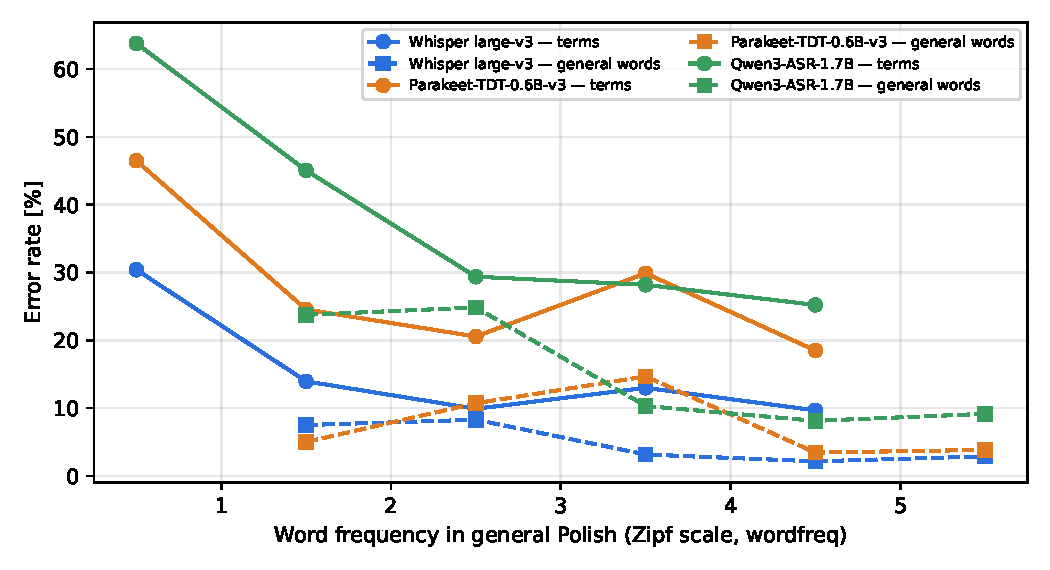
\includegraphics[width=0.78\textwidth]{fig_terms_vs_freq.pdf}
\caption{Odsetek błędów a częstość słowa w ogólnej polszczyźnie (skala Zipfa) dla terminów i słów ogólnych, dla trzech reprezentatywnych modeli. Przy tej samej częstości terminy są wyraźnie trudniejsze.}
\label{fig:zipf}
\end{figure*}

\section{Dyskusja}
\noindent\textbf{Klasyczny ASR a transkrybery oparte na LLM.} Wyniki dzielą systemy na dwie rodziny. Klasyczne systemy akustyczne traktują terminologię jak problem poza słownikiem: sygnał jest rozpoznawany, ale termin zapisywany jest jako fonetycznie prawdopodobny bliski zapis, dlatego TER/GWER jest wysoki, a dominuje bliski zapis. Transkrybery oparte na LLM (gpt-4o-transcribe, Gemini 3.5 Flash, a w ujęciu WER-N także ElevenLabs) wnoszą wiedzę leksykalną o pisowni i zmniejszają lukę. Ceną jest skłonność do „wygładzania'' (interpunkcja, podział wyrazów, wstawki), co surowy WER karze, ale lekarz może tolerować. Znormalizowany pod względem liczb WER oraz TER dają wierniejszy obraz użyteczności klinicznej niż sam zagregowany WER.

\noindent\textbf{Zapis liczb słownie to artefakt metryki.} ElevenLabs zapisuje liczby słownie, dając surowy WER 28,27\%, co błędnie sugerowałoby słaby system; jego WER-N 5,22\% lokuje go wśród najlepszych. Benchmarki polskiego (i innych języków o bogatej fleksji) dyktowania radiologicznego powinny podawać metrykę znormalizowaną pod względem liczb i wskazywać, której konwencji (cyfry czy słowa) wymaga wdrożenie.

\noindent\textbf{Liczy się nie zagregowany WER, lecz błędy krytyczne.} Kategorie krytyczne rozmijają się z rankingiem zagregowanym, a CCER je podsumowuje: prowadzi gpt-4o-transcribe (2,07\%), następnie Gemini 3.5 Flash (2,74\%), a ElevenLabs jest najryzykowniejszy w chmurze (65,56\%). Wybór modelu i przegląd przez człowieka powinny celować w liczby, zaprzeczenia i stronę ciała.

\noindent\textbf{Przewaga bliskich zapisów wskazuje na tanie lekarstwo.} Ponieważ większość błędów terminologicznych to bliskie zapisy, korekta leksykonowa lub lista terminów na etapie dekodowania mogłaby usunąć dużą część błędów bez treningu---górną granicę wyznacza różnica między TER (15,8\%) a TER-L (13,0\%) dla Whisper large-v3.

\section{Ograniczenia}
Zbiór testowy jest mały (2,69\,h), obejmuje dwie kategorie zdominowane przez USG tarczycy i składa się z czytanych fraz, a nie spontanicznego dyktowania, więc wyniki mogą nie przenosić się na pełne, swobodne opisy ani inne okolice ciała. Adnotację terminów wykonał model językowy, bez weryfikacji przez radiologa; granica termin/słowo ogólne jest umowna. Klasyfikacja bliskiego zapisu używa arbitralnego progu odległości edycyjnej, a surowy WER karze nieszkodliwe różnice formatowania (stąd WER-N i TER). Lokalny RTF zmierzono na jednej maszynie; RTF chmurowy nie jest bezpośrednio porównywalny. Kilku planowanych systemów nie udało się ocenić: Cohere Transcribe 03-2026 i NVIDIA Nemotron 3.5 Transcribe (gated lub wymagające wynajętego GPU), Soniox (brak środków na koncie), Google Chirp (wymaga projektu Google Cloud) i Azure AI Speech (brak klucza). Dedykowany model transkrypcyjny Google \texttt{gemini-3.5-transcribe} ma limit 100 żądań dziennie na pierwszym tierze, co uniemożliwia pełny przebieg w jednym dniu; zmierzono zamiast niego ogólny \texttt{gemini-3.5-flash}. Badanie mierzy systemy bez wsparcia (bez promptów ze słownictwem i korekty); wpływ takiego wsparcia to praca przyszła.

\section{Wnioski}
Gotowe systemy ASR są bliskie użyteczności do polskiego dyktowania radiologicznego, ale zagregowany WER ukrywa istotne klinicznie błędy. Na 939 nagraniach naturalnego głosu najlepszy model otwarty (Whisper large-v3) osiąga WER 8,03\%, ale myli 15,8\% terminów radiologicznych, 3--6$\times$ częściej niż słowa ogólne, z przewagą bliskich zapisów. Transkrybery oparte na LLM zmniejszają tę lukę: OpenAI gpt-4o-transcribe ma najlepszy ogólny WER (5,96\%) i CCER (2,07\%), a Google Gemini 3.5 Flash najlepszą poprawność terminów (TER 6,6\%). Zapis liczb może drastycznie zawyżać surowy WER, dlatego metryka znormalizowana pod względem liczb jest niezbędna; ElevenLabs Scribe v2 spada z 28,27\% surowego WER do 5,22\% WER-N. Ponieważ błędy koncentrują się w liczbach, zaprzeczeniach, stronie ciała i kilku skrótach, zarówno wybór modelu, jak i kontrola jakości powinny celować w te tokeny, a korekta leksykonowa jest obiecującym, tanim krokiem.

\section*{Dostępność danych i kodu}
Korpus ADMEDVOICE jest publiczny (Kaggle \texttt{karmarci/polish-medical-multi-source-corpus}, DOI 10.34740/kaggle/ds/6698205, licencja CC~BY~4.0) \cite{r1}. Kod ewaluacji, leksykon terminów oraz transkrypcje i metryki poszczególnych systemów udostępniono w repozytorium projektu (\url{https://github.com/kocasp/radiology_asr_research}); audio nie jest redystrybuowane i odtwarza się je z ADMEDVOICE skryptem \texttt{scripts/build\_radiology\_db.py}.

\section*{Odtwarzalność}
Do inferencji offline użyto PyTorch 2.15 (MPS), transformers 5.23 (Qwen3-ASR w osobnym środowisku), NVIDIA NeMo 3.0 oraz qwen-asr; metryki policzono bibliotekami jiwer, pyctcdecode 0.5 z KenLM, num2words, wordfreq 3.1.1 i simplemma 2.0. Analizę terminów odtwarza \texttt{uv run python terms.py} (Sekcja~V-C). Wszystkie przebiegi modeli lokalnych wykonano na MacBook Pro M1 Pro (16\,GB).

\begin{thebibliography}{99}
\bibitem{r1} A. Czyżewski et al., ``A Comprehensive Polish Medical Speech Dataset for Enhancing Automatic Medical Dictation,'' \emph{Scientific Data}, vol. 12, art. 1436, 2025. doi:10.1038/s41597-025-05776-1.
\bibitem{r2} A. Radford, J. W. Kim, T. Xu, G. Brockman, C. McLeavey, and I. Sutskever, ``Robust Speech Recognition via Large-Scale Weak Supervision,'' in \emph{Proc. ICML}, 2023. arXiv:2212.04356.
\bibitem{r3} A. Baevski, Y. Zhou, A. Mohamed, and M. Auli, ``wav2vec 2.0: A Framework for Self-Supervised Learning of Speech Representations,'' in \emph{Proc. NeurIPS}, 2020. arXiv:2006.11477.
\bibitem{r4} V. Pratap, A. Tjandra, B. Shi, et al., ``Scaling Speech Technology to 1,000+ Languages,'' 2023. arXiv:2305.13516.
\bibitem{r5} NVIDIA, ``Canary-1B-v2 model card,'' Hugging Face, 2025. \url{https://huggingface.co/nvidia/canary-1b-v2}
\bibitem{r6} NVIDIA, ``Parakeet-TDT-0.6B-v3 model card,'' Hugging Face, 2025. \url{https://huggingface.co/nvidia/parakeet-tdt-0.6b-v3}
\bibitem{r7} NVIDIA, ``Polish FastConformer hybrid (P\&C) model card,'' Hugging Face. \url{https://huggingface.co/nvidia/stt_pl_fastconformer_hybrid_large_pc}
\bibitem{r8} Qwen Team, ``Qwen3-ASR-1.7B model card,'' Hugging Face, 2026. \url{https://huggingface.co/Qwen/Qwen3-ASR-1.7B}
\bibitem{r9} J. Grosman, ``wav2vec2-large-xlsr-53-polish model card,'' Hugging Face. \url{https://huggingface.co/jonatasgrosman/wav2vec2-large-xlsr-53-polish}
\bibitem{r10} Google, ``MedASR model card,'' Hugging Face. \url{https://huggingface.co/google/medasr}
\bibitem{r11} OpenAI, ``Audio transcription API (whisper-1, gpt-4o-transcribe),'' Documentation, 2026. \url{https://platform.openai.com/docs}
\bibitem{r12} ElevenLabs, ``Speech-to-text (Scribe) documentation,'' 2026. \url{https://elevenlabs.io/docs}
\bibitem{r13} Deepgram, ``Nova-3 documentation,'' 2026. \url{https://developers.deepgram.com}
\bibitem{r14} AssemblyAI, ``Documentation,'' 2026. \url{https://www.assemblyai.com/docs}
\bibitem{r15} Speechmatics, ``Documentation,'' 2026. \url{https://docs.speechmatics.com}
\bibitem{r16} Google, ``Gemini API documentation,'' 2026. \url{https://ai.google.dev/gemini-api/docs}
\bibitem{r17} T. Wolf, L. Debut, V. Sanh, et al., ``Transformers: State-of-the-Art Natural Language Processing,'' in \emph{Proc. EMNLP (system demonstrations)}, 2020. arXiv:1910.03771.
\bibitem{r18} A. C. Morris, V. Maier, and P. Green, ``jiwer: Evaluate ASR output,'' GitHub. \url{https://github.com/jitsi/jiwer}
\bibitem{r19} Kensho Technologies, ``pyctcdecode,'' GitHub. \url{https://github.com/kensho-technologies/pyctcdecode}
\bibitem{r20} K. Heafield, ``KenLM: Faster and Smaller Language Model Queries,'' in \emph{Proc. WMT}, 2011.
\bibitem{r21} R. Speer, J. Chin, and A. Lin, ``wordfreq,'' GitHub, 2018. \url{https://github.com/rspeer/wordfreq}
\bibitem{r22} A. Barbaresi, ``simplemma,'' GitHub. \url{https://github.com/adbar/simplemma}
\bibitem{r23} Savoir-faire Linux, ``num2words,'' GitHub. \url{https://github.com/savoirfairelinux/num2words}
\bibitem{r24} G. K. Zipf, \emph{Human Behavior and the Principle of Least Effort}. Addison-Wesley, 1949.
\end{thebibliography}

\end{document}
